\subsection{Technical and Financial Context}

There are four underlying storage trends that affect the acquisition, storage and utilisation of weather and climate data: 
\begin{enumerate}
\item The rise of NAND storage as a competitor for spinning disk,
\item The advent of NVRAM associated ``burst buffer'' solutions in HPC,
\item The advent of object store technology as cost effective and performant disk store, and
\item physical limits on storage and bandwidth of (spinning) disk and tape.
\end{enumerate}

These trends affect both economics and performance, and will have profound affects on workflow both in the near future, and in the medium to longer term future as 
the community embraces exabytes of data, and then, exaflop computers.  
They will also have profound impacts on cost, and as such, the architecture of future data centres will be increasingly driven by economic realities, as well, as 
received wisdom\footnote{``received wisdom'': knowledge or information that people generally believe is true, although in fact it is often false 
(\url{http://idioms.thefreedictionary.com/the+received+wisdom}). }
as to how best to exploit existing technologies. However, one of the problems with such wisdom is that it is often developed in very different environments, and may 
not be applicable to petascale, let alone exascale, weather and climate workflows. For example, while the internet giants currently handle exabytes of data, and 
deploy data mining, they do not typically handle multiple data workflows which themselves approach petascale, rather they typically handle millions of simultaneous 
megascale workflows, or handle data mining problems with gigabytes to terabytes of source data. For these reasons, their technical solutions are optimised for very 
different performance and price strategies. Hence, to examine the right computing environment for peta to exascale weather and climate workloads, basic research 
on cost/benefit ratios and possible technical strategies is necessary.

The difficulty of this basic research is compounded by the zoo of technical options available, and in particular, by the potential issues associated with multiple levels 
of storage with concomitant cache and performance characteristics. Because of this, it is often hard to estimate the cost and plan future data centres, particularly as 
we aim towards the exascale. In part this can be attributed to the limited availability and scattered nature of data on unit storage costs and performance as well as 
the lack of models for simulating the interactions between the various components found in modern data centres.  

For example, conventional hard drives provide good storage density, but decreasing ``access density'' (as capacity
increases much faster than read/write speeds). By contrast, the advent of storage class memory, non-volatile memory technologies, and flash arrays provide new opportunities for supporting high-speed access, but are expensive at scale. Similarly, tape is relatively cheap, but access latency is poor.  So it is very likely that future data centres will combine these technologies into storage hierarchies, but how does one make decisions about the architectures? 

The choice of technical options is directly related to enterprise organisational objectives, which are themselves subject to political decisions. For example, in the UK, 
the storage and analysis facility for academic climate science (JASMIN) is physically located in one part of the country (Oxfordshire), while the HPC simulation 
engines (ARCHER and MONSOON) are located in others (Edinburgh and Exeter respectively). The situation is similar for the US Geophysical Fluid Dynamics 
Laboratory (GFDL) who have their storage and analysis facility in Princeton NJ, but most of their simulations are done at Oak Ridge National Laboratory (Oak 
Ridge, TN). By contrast, the UK Met Office and the German Climate Computing Center (DKRZ) have co-located compute, storage and analysis facilities, although 
both make use of remote HPC as well. 

\begin{figure}
\centering
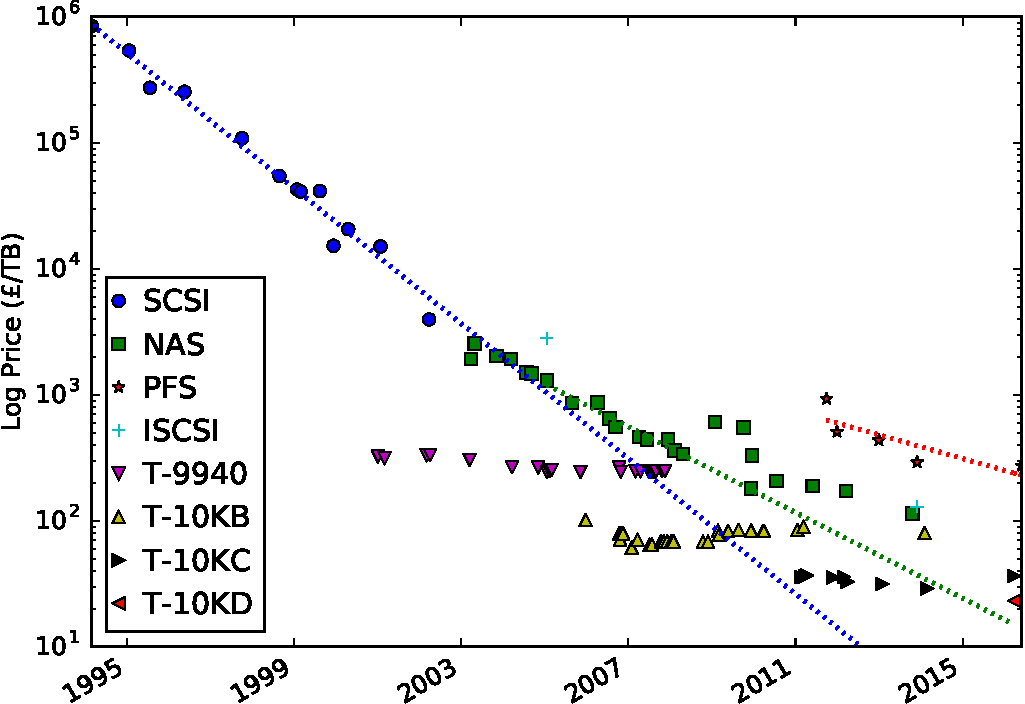
\includegraphics[width=0.8\linewidth]{3rd/kryder_2016.pdf}
\caption{Twenty years of storage costs at the STFC Centre for Environmental Data Analysis. Four distinct disk based architectures are shown, and four generations 
of tape technology. There is not enough use of ISCSI disk data to draw conclusions, but it can be seen that in the early years, the use of SCSI disk followed a linear 
trend which would have resulted in disk costing less than \pounds 1 TB in 2017 ... a trend that could not be sustained, in part because while disk densities have 
grown, the need for more and more disks has meant more and more of the storage budget needs to be spent on the kit (hardware and software) which surrounds the 
disks. The trend from the early NAS years was clearly not sustained. The advent of parallel file systems (PFS) at CEDA followed the recognition that it was not 
possible to manage or deliver the requisite performance with NAS based disk. It is too early to believe the trend in costs associated with PFS, but it is also clear that 
whatever trend might exist, will not be sustainable. The net conclusion is that the experience of disk getting cheap quickly which has provided the received wisdom 
over the last two decades that future growth in data volume will be compensated by falling costs for storage is no longer true. Disk is getting cheaper, but not as 
quickly as data volumes for storage are growing.  The advent of object store technologies will lead to a new set of data, but is unlikely to change the conclusion.
The tape storage costs also show that it is really only a change in technology that leads to substantial changes in tape media costs.
\label{fig:kryder}}
\end{figure}

In addition,  many academic/research data centres will need to support multi-disciplinary research, and will achieve economy of scale
by supporting multiple science/research areas.  A data centre run by the likes of DKRZ, the Met Office, or ECMWF can
afford to focus entirely on supporting climate research, whereas a data centre run by an organization with a wider
research base such as STFC, ORNL, or NERSC will need to support other activities, and can in fact sometimes benefit from supporting
other activities, e.g., through economy of scale.  By contrast, dedicated facilities can exploit simplifications; it can be assumed that
data contains no personal data and no sensitive data, meaning that encryption and tight access control does not need to be
 a priority within the system, and de-duplication is unlikely to be worth the investment. It might be  possible to establish workflows
 and polices which allow ``deep archival'' with data migration between cold/warm and hot storage for further analysis (and regular fixity checks).
 
In all cases there are direct trade-offs between the amount of compute and storage, and even within that, the amount and 
configuration with respect to types of usage (simulation versus analysis). 
Not all trade-offs are well understood in terms of cost/performance and scientific benefits.

One key trade-off is of course cost. Over the long-term, the fall in storage cost for disk, known as Kryder's Law has not been as linear as received wisdom expects 
(see \Cref{fig:kryder}), and while tape media costs have fallen in the long term, and over time they are generally much cheaper than disk, at times they have not 
been substantially cheaper than raw disk. These lessons: that disk is not getting as cheap as quickly as it used to, and that tape media costs are generally 
significantly less than disk, are not well known, and one of the drivers of this work will be establishing and promulgating the relevant modelling.

%
% I don't know who wrote this, but i find it offensive :-) ... as if BADC and DKRZ were not world leaders (ahead of, or 
% often in partnership with humanities and digital libraries, but certainly not behind).
%
%The multidisciplinary approach applies also to data, where, for example, humanities and digital libraries have for
%decades led the way in long term preservation and curation of data, and these activities could be brought to bear on
%climate data --- even if there were no immediate need for curation, we shall see that with increasing data volumes, it
%will become necessary to apply methodologies from preservation to ensure fixity of data.  Similar features from
%humanities (and elsewhere) which will become increasingly important include provenance, supporting processes for QA,
%and, possibly, annotations.



As well as the fundamentals of storage technology, there are other major components of systems which need to be considered. In particular,
\begin{itemize}
\item Interfaces:  The need to either develop hybrid data solutions or connected homogeneous solutions, which are fit for the workflows currently in use.  As noted 
above, this can include data migration over wide-area networks, and significant variations in how compute and storage are organised. This means storage solutions 
need to be suitable for linking to to research infrastructures that support both local and remote research institutes. They need to support data replication between 
sites (or tiers of storage), links to cloud service providers, and potentially complicated licensing regimes.  All these use-cases require standardised interfaces.
\item Automation:  Anything that doesn't happen by itself needs a human to do it.  Without automation, staff
  with the right skills and privileges need to be on hand to fix it.  While there will always be tasks that cannot be
  automated, automation of tasks helps free staff for more important tasks, and overall reduces the staff costs of the
  data centre. With increasing scale comes increasing requirement for automation, and technology choices which require
  manual intervention become unfeasible - no matter how cheap and performant they may be (it is this transition of scale, performance, and need for automation that 
led to each of the disk technology changes  shown in figure \ref{fig:kryder}).
\item Policy Support: Given the likelihood of requiring multiple levels of storage, support for effective policy management will be necessary. Support that includes 
both automatic data migration and the requirements of both system managers and users (who must be able to use their knowledge of what is important, and likely to 
be hot or cold data, to inform automatic data systems). 
  give hints or requirements on the desired features. 
\item Software:  The need for automation will also require customisation.  All storage solutions will need to support customised workflows by appropriate application 
programming interfaces. 
\end{itemize}
